\section{Experimental Results and Discussion}

As a reference, we compared our best results for each task with their corresponding benchmarks (Table\ref{benchmark}). 
For POS-tagging and chunking, we reach a comparable performance to the state-of-the-art methods.
The difference between our NER system and its baseline is most obvious, as we are 0.025 points below them, but the comparison is not fair considering that their algorithm is much complex
(\newcite{Ando:2005} used a $2^{nd}$ order CRF, while we used a $1^{rst}$ order CRF).
%, which use as features the two previous predictions and the previous label combined with the current word).
For the task of MWE identification, our implementation and settings beat the baseline. 
However, in this paper, we do not aim to maximize the absolute performance of the tasks under 
study, but rather to study the impact of word embeddings for sequence tagging tasks under control settings. 
Accordingly, we focus in addressing the following questions:

\begin{table*}
\caption{Benchmark results vs. our best results}
\begin{center}
\begin{small}
\begin{tabular}{lll}
\hline
\textbf{Task} & \textbf{Benchmark} & \textbf{Us} \\ \hline
POS-Tagging & (Accuracy) 97.24 \cite{Toutanova:2003} & 0.9592 (skip-gram negsam+up) \\ 
Chunking & (F1) 0.9429 \cite{Sha:2003} & 0.9386 (Brown cluster v2000+)\\  
NER & (F1) 0.8931 \cite{Ando:2005} & 0.8686 (skip-gram negsam+noup)\\  
MWE & (F1) 0.6253 \cite{Schneider+:2014} & 0.6546 (cw+up)\\ 
\hline
\label{benchmark}
\end{tabular}
\end{small}
\end{center}
\end{table*}


\textbf{(i) Are the evaluated word embedding methods better than unigram features?}
To answer this question, we systematically compared the usefulness of word embedding versus
unigram features for sequence tagging and noted that word embedding methods always outperform 
unigram features (Figures \ref{fig:bestPOS-Chunk}, \ref{fig:bestNER-MWE}). 

\textbf{(ii) How does the size of labelled training data affect the experimental results?}
We observed that embedding methods are especially helping POS-tagging and chunking when there are only several hundreds of training instances. 
Therefore, confirming that any of the evaluated word embedding methods should be use when labelled data is limited.
These early improvements are less evident for NER and MWE. 
We attribute this to: a) NER and MWE are more difficult tasks than POS-tagging and chunking;
b) NER and MWE require more training data to reach a decent performance; c) the performance of NER and MWE heavily dependent on complex features such as gazetteers and lexicons like Wordnet, which are not captured by the feature representation learned from unlabelled data, meanwhile the standard features used in POS-tagging and chunking (e.g., context words, stemmed words) are similar to the representations encoded in the word embeddings.

\textbf{(iii) How well do the word embeddings perform for unknown words?}
As already mentioned, we measure the performance for out-of-vocabulary words (OOV)
in two settings: with \textit{in-domain} and \textit{out-of-domain} corpora, for all the tasks, except MWE identification for which there is no other data set available (see Table \ref{datasplit}).
As expected, word embeddings and Brown clustering excel in \textit{out-of-domain} performance.
Word embeddings without fine-tuning enhance even more the performance of OOV 
for the \textit{in-domain} and \textit{out-of-domain} settings (Figure \ref{OOV}) since fine-tuned
word representations become task-specific, hence performing worst for OOV.

%\textbf{(iv) How do the key parameters of each word learning algorithms affect the experimental results?} 

\textbf{(iv) How well do different word embeddings perform in all tasks when semi-supervised fine-tuning is not performed?}, and 
\textbf{(v) and how well do different word embeddings perform in all tasks when semi-supervised fine-tuning is performed?}
%According to our results, there is not a clear trend about fine-tuning or not during training. 
Across all the methods, fine-tuning is helping POS-Tagging and MWE, where the CW method has been found to be the most sensible to tuning, reaching almost 3 points more, when tuning is performed. 
For chunking and NER, the best results are fine-tuned, but the difference across all the methods and updated features versus not-updated ones, is not significant. 
We also found that fine-tuning can correct poorly learned word representations but can be
overfitted if unsupervisely learned ones are already good. 

Finally, we address the following question: \textbf{(vi) It has been shown that Brown clusters are useful features for MWE identification but, are also word embeddings helping MWE identification?} 
According to our experiments, the word embedding features distilled by fine-tuned CW reached the best results, beating the state-of-the-art performance (see Table \ref{benchmark}).
However, between Brown clusters and fine-tuned CW, learned under the same settings, the difference is not impressive, suggesting that distributional word representations and cluster-based representations captures similar features for the MWE identification task.
Thus, a natural question: would it be better to learn distributional representations for MWE, instead of representations of single words?




%%%%%%%%%%%%%%%%%%%%%%%%%%%%
%%% HEATMAPS 


\begin{figure*}
\caption{Best results for each method for POS-Tagging and Chunking. The x-axis correspond to the different word embeddings methods and the y-axis to the 10 training partitions at log scale. Green color stand for high performance, while red color stands for low performance. The methods are in chronological order}
\centering
\begin{subfigure}{7cm}
	\centering
    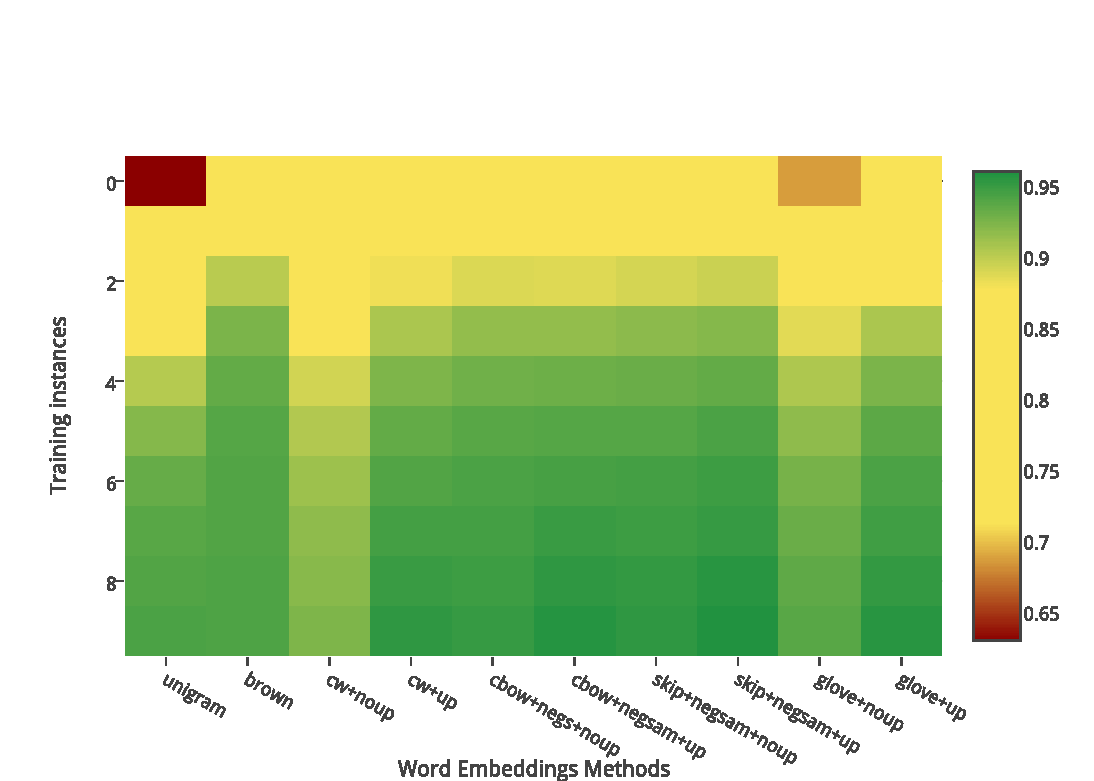
\includegraphics[scale=0.4]{plots/map-pos}    	
	\subcaption{POS-Tagging Accuracy}	
\end{subfigure}
\begin{subfigure}{7cm}
	\centering
    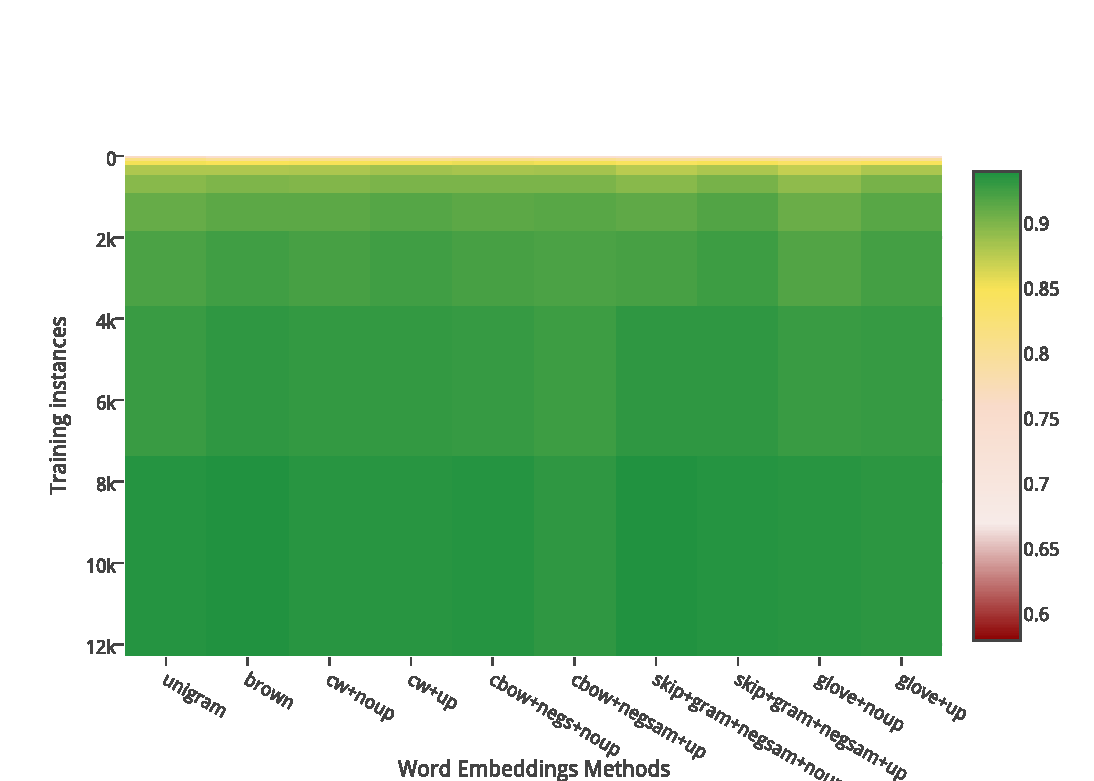
\includegraphics[scale=0.4]{plots/map-chunk}
	\subcaption{Chunking F1-Measure}	
\end{subfigure}
\label{fig:bestPOS-Chunk}
\end{figure*}

\begin{figure*}
\caption{Best results for each method for NER and MWE}
\centering
\begin{subfigure}{7cm}
	\centering
    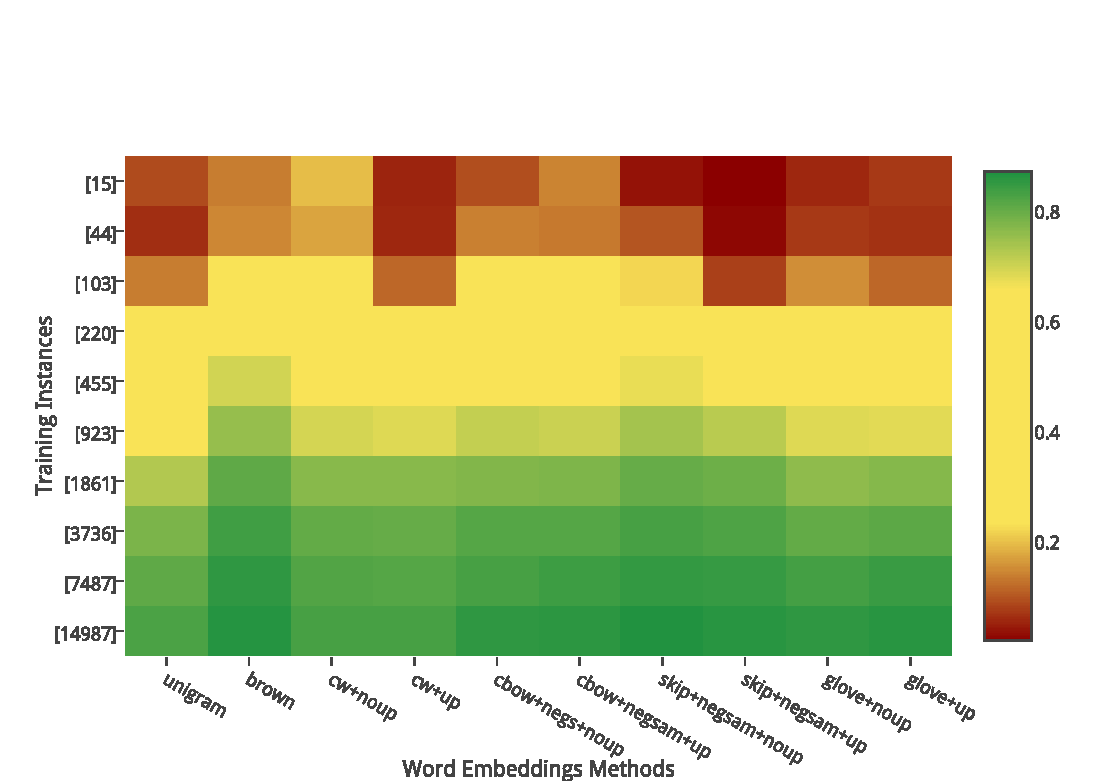
\includegraphics[scale=0.4]{plots/map-ner}    	
	\subcaption{NER F1-Measure}	
\end{subfigure}
\begin{subfigure}{7cm}
	\centering
    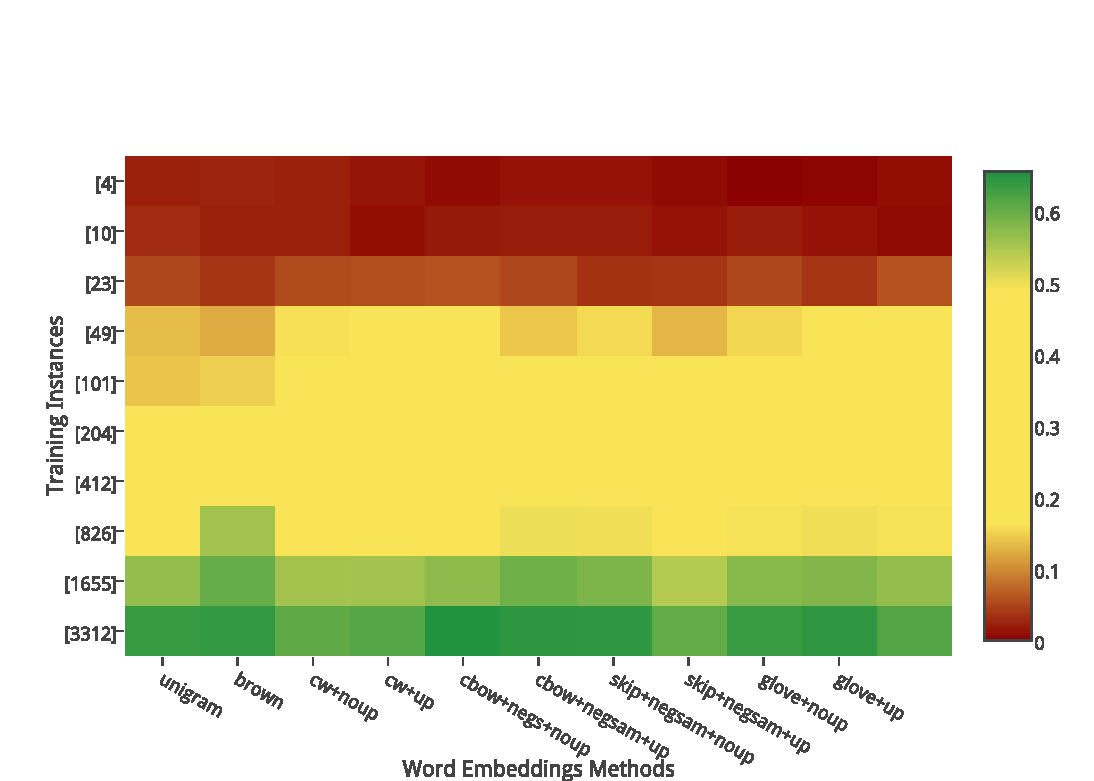
\includegraphics[scale=0.4]{plots/map-mwe}
	\subcaption{MWEs F1-Measure}		
\end{subfigure}
\label{fig:bestNER-MWE}
\end{figure*}






\iffalse
%%%%%%%%%%%%%%%%%%%%%%%%%%%%
%%% BEST in PLOTS
\begin{figure*}[h]
\caption{Best results for each method for POS-Tagging and Chunking}
\centering
\begin{subfigure}{6cm}
	\centering
    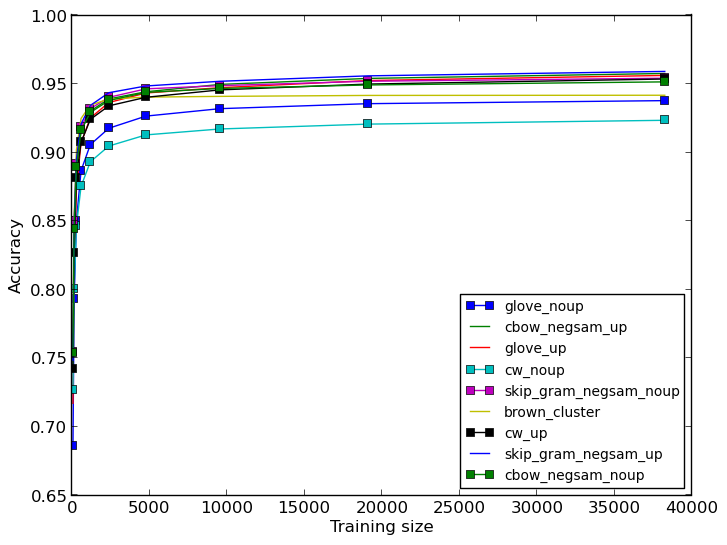
\includegraphics[scale=0.3]{plots/bestPOS}    	
	\label{fig:bestpos}
	\subcaption{POS-Tagging results}	
\end{subfigure}
\begin{subfigure}{6cm}
	\centering
    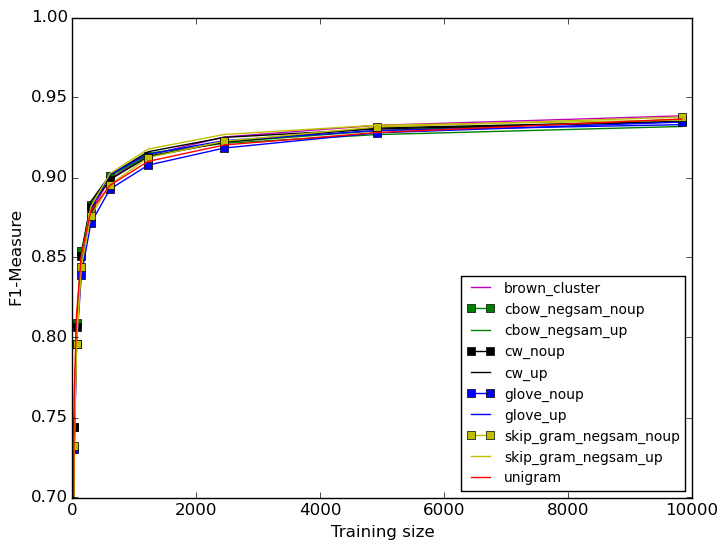
\includegraphics[scale=0.3]{plots/bestChunking}
	\label{fig:bestchunking}
	\subcaption{Chunking results}	
\end{subfigure}
\end{figure*}

\begin{figure*}[h]
\caption{Best results for each method for NER and MWE}
\centering
\begin{subfigure}{6cm}
	\centering
    	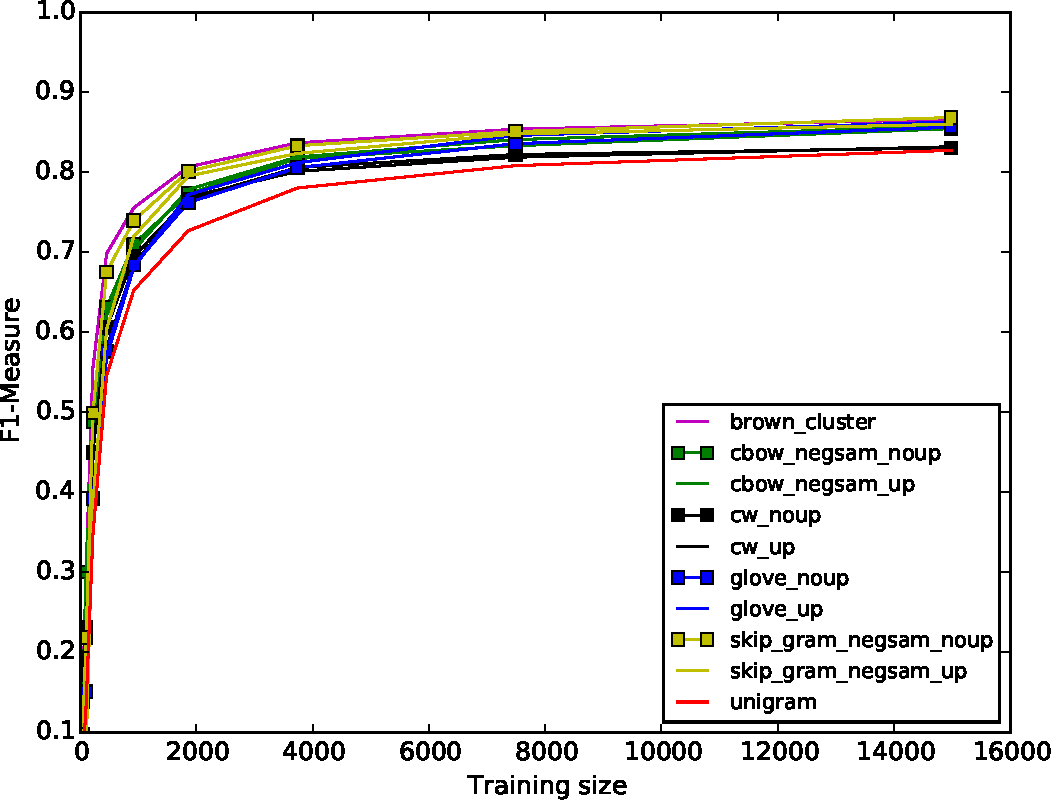
\includegraphics[scale=0.3]{plots/bestNER}
	\subcaption{NER results}	
	\label{fig:bestner}
\end{subfigure}
\begin{subfigure}{6cm}
	\centering
    	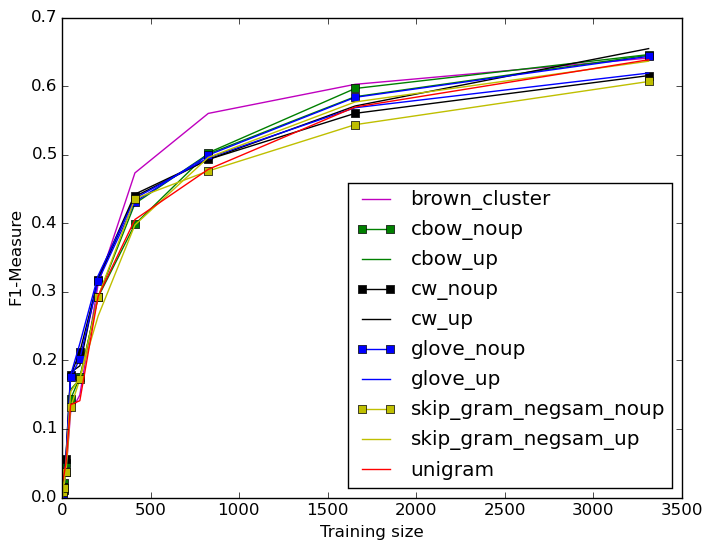
\includegraphics[scale=0.3]{plots/bestMWE}
    \subcaption{MWE results}	
	\label{fig:bestmwe}
\end{subfigure}  	
\end{figure*}  

\begin{figure*}[h]
\caption{Chunking and MWE out-of-vocabulary-words accuracy for \textit{in-domain} test set}
\centering
\begin{subfigure}{7cm}
	\centering
    	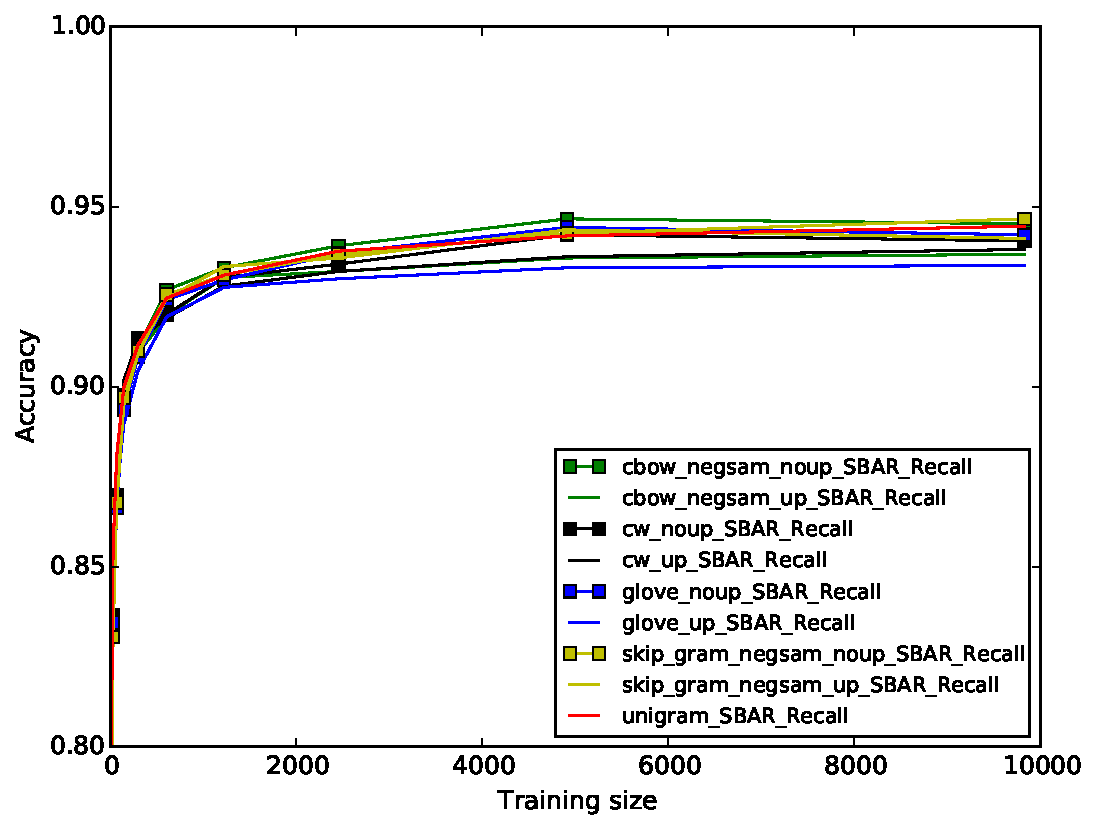
\includegraphics[scale=.4]{plots/Chunking-OOV}
    	\subcaption{Chunking accuracy for OOV}
	\label{fig:inner}
\end{subfigure}
\begin{subfigure}{7cm}
	\centering
    	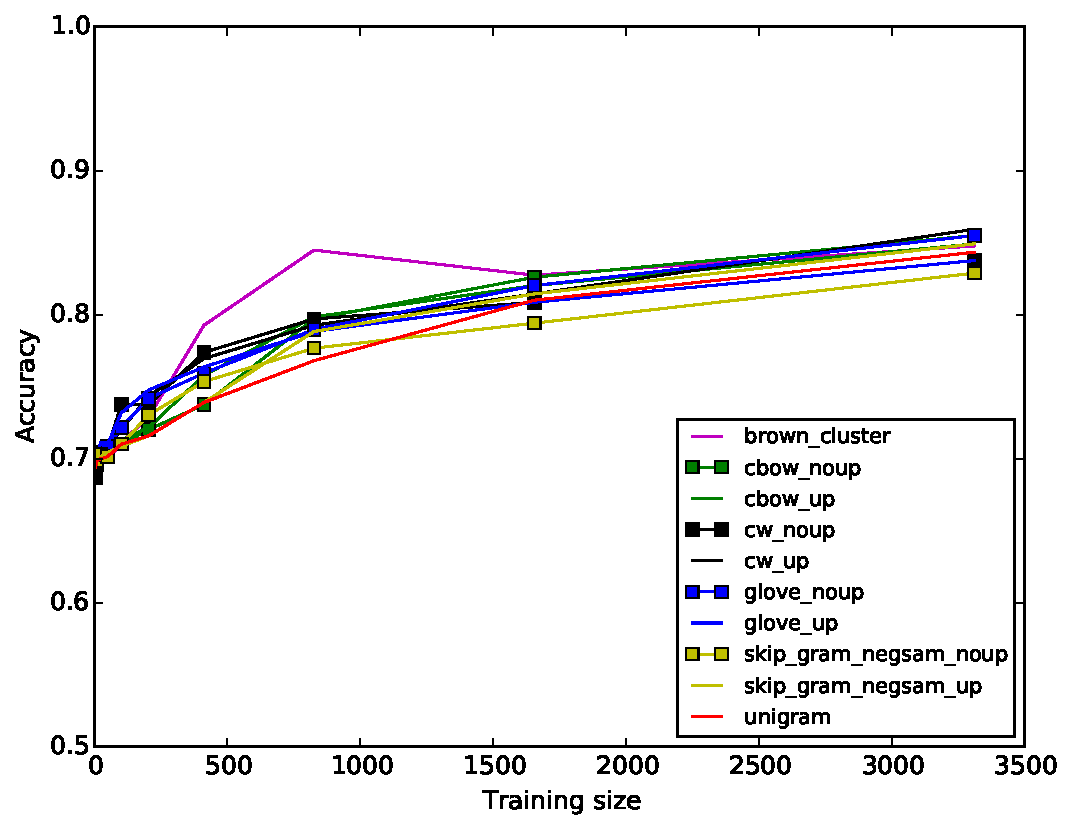
\includegraphics[scale=0.4]{plots/MWE-OOV}
   	\subcaption{MWE accuracy for OOV}
	\label{fig:outner}
\end{subfigure}  	
\end{figure*}	
\fi



%%%%%%%%%%%%%%%%%%%%%%%%%%%%
%%% OOV POS and NER
\begin{figure*}
\caption{Out-of-vocabulary-words (OOV) accuracy for \textit{in-domain} and \textit{out-of-domain} test sets}
\label{OOV} 
  \begin{minipage}[b]{7cm}
    	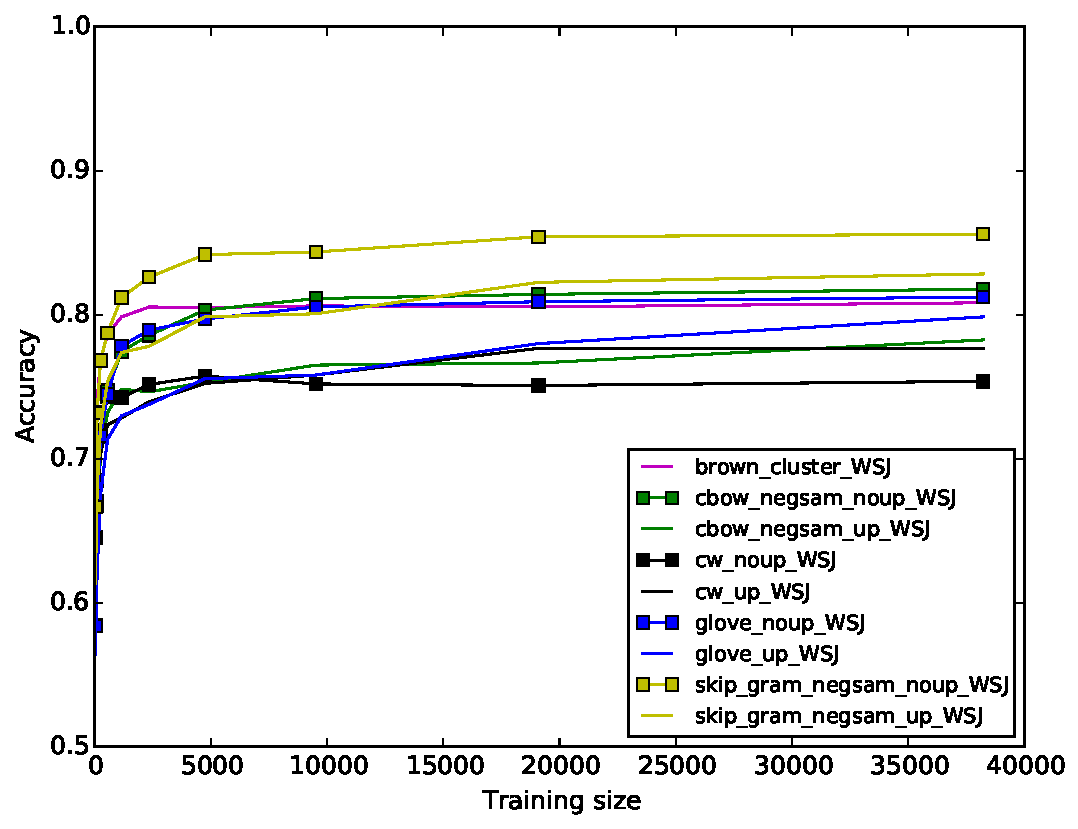
\includegraphics[scale=0.4]{plots/POS-OOV-IN}
    \subcaption{POS-Tagging accuracy for \textit{in domain} OOV} 
    \label{POS-OOV-IN}	
  \end{minipage} 
  \begin{minipage}[b]{7cm}
    	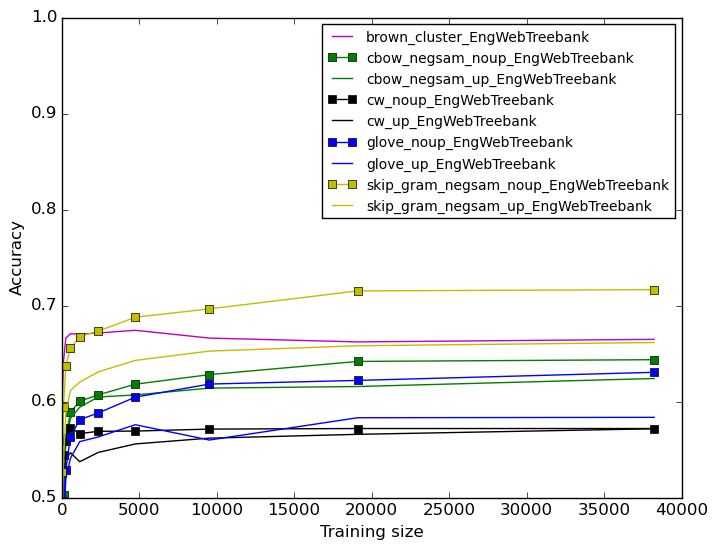
\includegraphics[scale=0.4]{plots/POS-OOV-OUT}
    \subcaption{POS-Tagging accuracy for \textit{out domain} OOV} 
    \label{POS-OOV-OUT}	
  \end{minipage} 
  \begin{minipage}[b]{7cm}
    	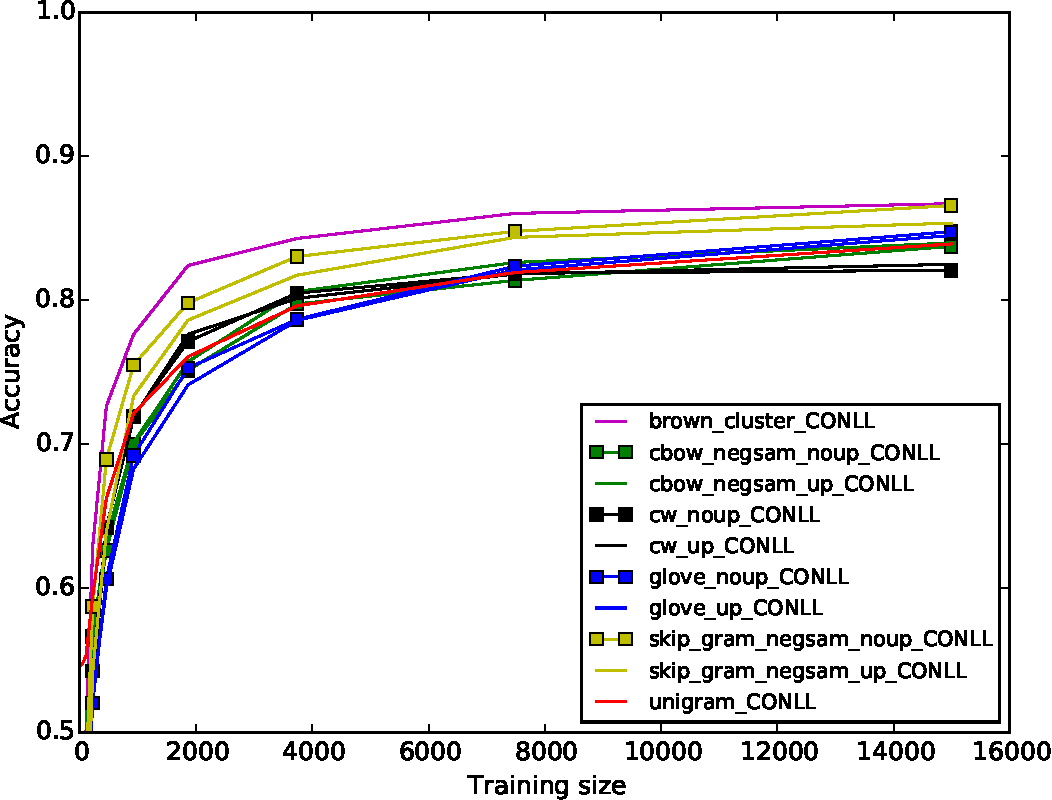
\includegraphics[scale=0.4]{plots/NER-OOV-IN}
    \subcaption{NER accuracy for \textit{out domain} OOV} 
    \label{NER-OOV-IN}
  \end{minipage}
  \hfill
  \begin{minipage}[b]{7cm}
    	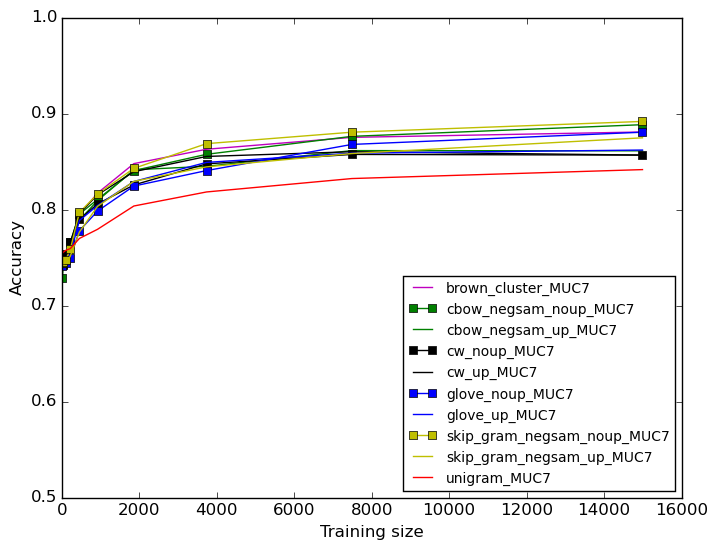
\includegraphics[scale=0.4]{plots/NER-OOV-OUT}
    \subcaption{NER accuracy for \textit{out domain} OOV} 
    \label{NER-OOV-OUT}
  \end{minipage} 
  \begin{minipage}[b]{7cm}
    	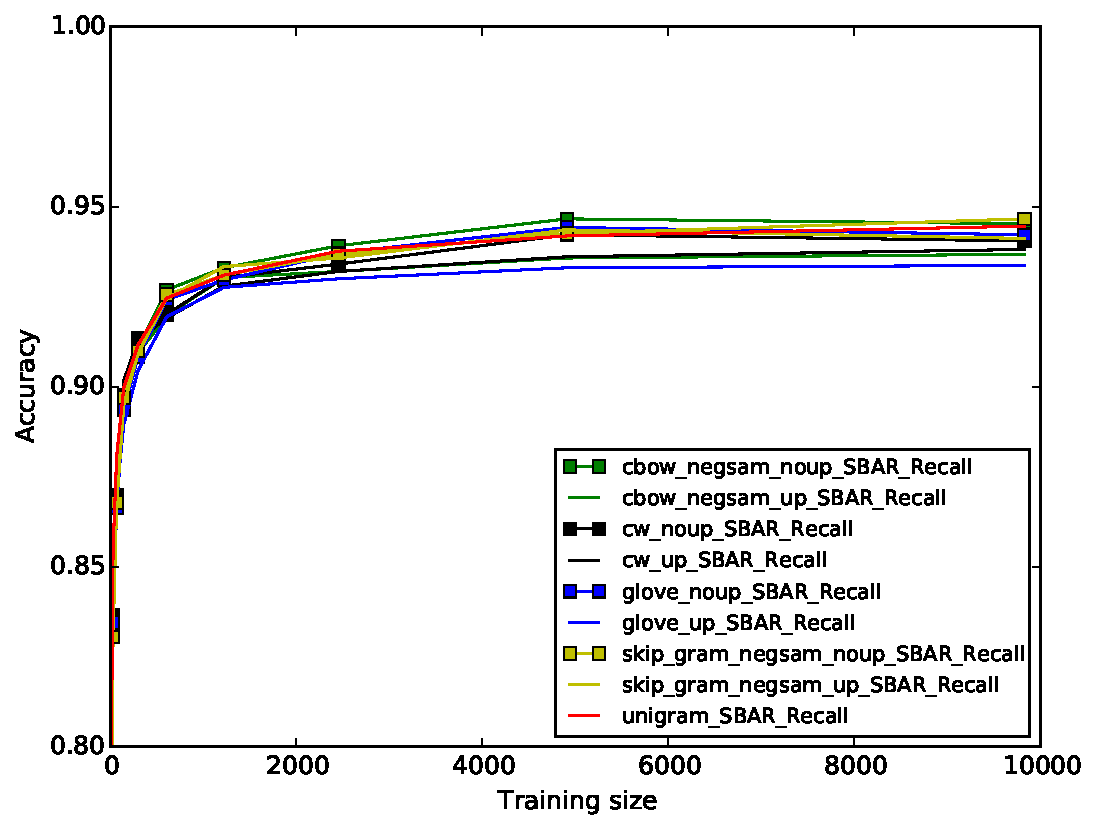
\includegraphics[scale=0.4]{plots/Chunking-OOV}
    \subcaption{Chunking accuracy for OOV \textit{in domain} OOV} 
    \label{chunk-OOV}
  \end{minipage} 
    \hfill
  \begin{minipage}[b]{7cm}
    	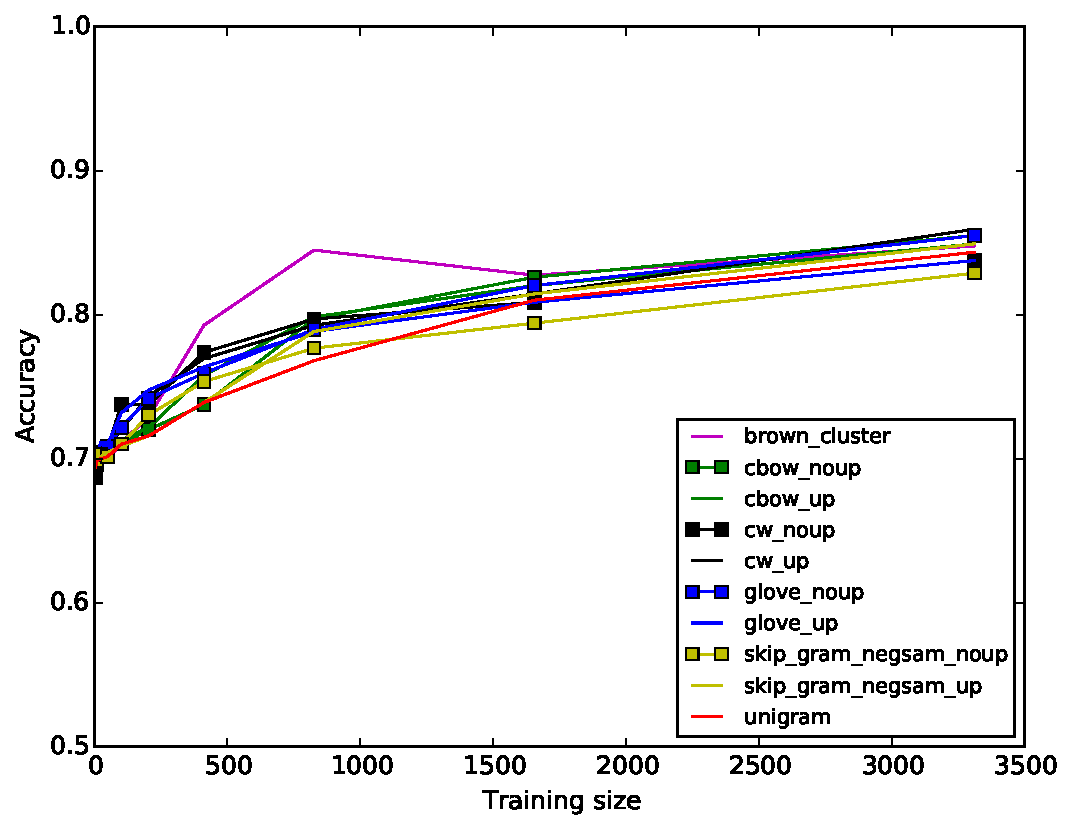
\includegraphics[scale=0.4]{plots/MWE-OOV}
     \label{POS-OOV}
    \subcaption{MWE accuracy for \textit{in domain} OOV} 
  \end{minipage}   
\end{figure*}


\iffalse
\subsection{Result tables}
The first column of each table contains the number of training sentences.
\subsubsection{Best hyperparameters for All Tasks}

\begin{table*}[h]
\centering
\begin{adjustbox}{max width=\textwidth}
\pgfplotstabletypeset[col sep=comma, 
precision=4,
every head row/.style={
before row=\toprule,
after row=\midrule},
every last row/.style={
after row=\bottomrule
}]{eval_results/key_results/POS/Accuracy.csv}
\end{adjustbox}
\caption{Accuracy of POS tagging evaluated on WSJ test set}
\label{table:accuracy_pos}
\end{table*}

\begin{table*}[h]
\centering
\begin{adjustbox}{max width=\textwidth}
\pgfplotstabletypeset[col sep=comma, 
precision=4,
every head row/.style={
before row=\toprule,
after row=\midrule},
every last row/.style={
after row=\bottomrule
}]{eval_results/key_results/NER/CONLL_F1Measure.csv}
\end{adjustbox}
\caption{F1 Measure of NER evaluated on CoNLL test set}
\label{table:f1_ner}
\end{table*}

\begin{table*}[h]
\centering
\begin{adjustbox}{max width=\textwidth}
\pgfplotstabletypeset[col sep=comma, 
precision=4,
every head row/.style={
before row=\toprule,
after row=\midrule},
every last row/.style={
after row=\bottomrule
}]{eval_results/key_results/chunking/chunks_F1Measure.csv}
\end{adjustbox}
\caption{F1 Measure of chunking evaluated on CoNLL test set}
\label{table:f1_chunking}
\end{table*}

\begin{table*}[h]
\centering
\begin{adjustbox}{max width=\textwidth}
\pgfplotstabletypeset[col sep=comma, 
precision=4,
every head row/.style={
before row=\toprule,
after row=\midrule},
every last row/.style={
after row=\bottomrule
}]{eval_results/key_results/MWEs/mwe_F1Measure.csv}
\end{adjustbox}
\caption{F1 Measure of MWE identification evaluated on MWE test set}
\label{table:f1_mwe}
\end{table*}

\subsubsection{Out of Vocabulary results for All Tasks}

\begin{table*}[h]
\centering
\begin{adjustbox}{max width=\textwidth}
\pgfplotstabletypeset[col sep=comma, 
precision=4,
every head row/.style={
before row=\toprule,
after row=\midrule},
every last row/.style={
after row=\bottomrule
}]{eval_results/key_results/POS/WSJ_out-of-vocabulary_Accuracy.csv}
\end{adjustbox}
\caption{Accuracy of POS tagging evaluated on out-of-vocabulary words in WSJ test set}
\label{table:outVocab_pos_accuracy}
\end{table*}

\begin{table*}[h]
\centering
\begin{adjustbox}{max width=\textwidth}
\pgfplotstabletypeset[col sep=comma, 
precision=4,
every head row/.style={
before row=\toprule,
after row=\midrule},
every last row/.style={
after row=\bottomrule
}]{eval_results/key_results/NER/CONLL_out-of-vocabulary_Accuracy.csv}
\end{adjustbox}
\caption{Accuracy of NER evaluated on out-of-vocabulary words in CoNLL test set}
\label{table:outVocab_ner_accuracy}
\end{table*}

\begin{table*}[h]
\centering
\begin{adjustbox}{max width=\textwidth}
\pgfplotstabletypeset[col sep=comma, 
precision=4,
every head row/.style={
before row=\toprule,
after row=\midrule},
every last row/.style={
after row=\bottomrule
}]{eval_results/key_results/chunking/Accuracy.csv}
\end{adjustbox}
\caption{Accuracy of Chunking evaluated on out-of-vocabulary words in CoNLL test set}
\label{table:outVocab_chunking_accuracy}
\end{table*}

\begin{table*}[h]
\centering
\begin{adjustbox}{max width=\textwidth}
\pgfplotstabletypeset[col sep=comma, 
precision=4,
every head row/.style={
before row=\toprule,
after row=\midrule},
every last row/.style={
after row=\bottomrule
}]{eval_results/key_results/MWEs/out-of-vocabulary_Accuracy.csv}
\end{adjustbox}
\caption{Accuracy of MWE identification evaluated on out-of-vocabulary words in MWE test set}
\label{table:outVocab_mwe_accuracy}
\end{table*}

\subsubsection{Out of domain Results for NER and POS}

\begin{table*}[h]
\centering
\begin{adjustbox}{max width=\textwidth}
\pgfplotstabletypeset[col sep=comma, 
precision=4,
every head row/.style={
before row=\toprule,
after row=\midrule},
every last row/.style={
after row=\bottomrule
}]{eval_results/key_results/POS/EngWebTreebank_Accuracy.csv}
\end{adjustbox}
\caption{Accuracy of POS tagging evaluated on English web treebank.}
\label{table:outDomain_accuracy_pos}
\end{table*}

\begin{table*}[h]
\centering
\begin{adjustbox}{max width=\textwidth}
\pgfplotstabletypeset[
col sep=comma, 
precision=4,
every head row/.style={
before row=\toprule,
after row=\midrule},
every last row/.style={
after row=\bottomrule
}]{eval_results/key_results/NER/MUC7_chunks_F1Measure.csv}
\end{adjustbox}
\caption{F1 measure of NER evaluated on MUC7 test set}
\label{table:outDomain_ner_f1}
\end{table*}

\fi
